\documentclass{beamer}

\usetheme{Copenhagen}
\usepackage{listings}

\title{Implementation and comparison of local search algorithms applied to the eight queens puzzle}

\author{Francesco Esposito}

\institute {
  Facolty of Computer Engineering \\
  Università degli studi di Napoli "Federico II"
}

\date{June 2024}
    
\begin{document}
    \frame{\titlepage}
    
    \begin{frame}
    \frametitle{Introduction}
    \pause
        \begin{itemize}
            \item Goal: Solve eigth queen puzzle using different local search algorithms.
            \pause
            \begin{itemize}
                \item Proprieties and performance of algorithms are also discussed.
            \end{itemize}
            \pause
            \item How? Using Python for the implementation and "Artificial Intelligent: A Modern approach (third edition)" as a reference.
            \pause
            \begin{itemize}
                \item Code will be avaiable on Github (on francespos account) after the exam.
            \end{itemize}
        \end{itemize}
    \end{frame}

    \begin{frame}
    \frametitle{The eigth queens puzzle}
        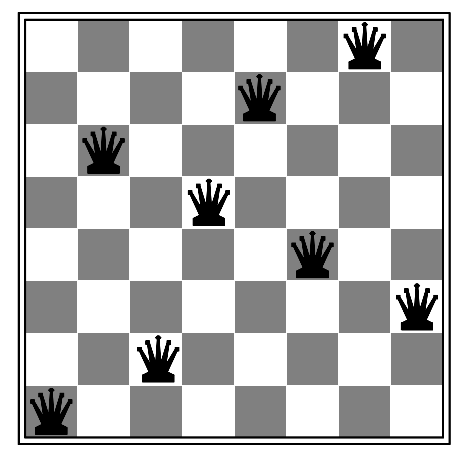
\includegraphics[scale=0.5]{Images/8_queens_puzzle.png}
        \centering
    \end{frame}

    \begin{frame}
    \frametitle{The eigth queens puzzle}
    \begin{itemize}
        \item Problem: place eigth queens on a chessboard so that they don't attack each other.
        \pause
        \item Rules: A queen can move horizontally, vertically and diagonally within an arbitrary range.
        \pause
            \begin{itemize}
                \item We will ignore states where queens are in the same row or in the same colon, because they can't belong to the solution.
            \end{itemize}
        \pause
        \item We will use PEAS approach to describe the problem.
    \end{itemize}
    \end{frame}

    \begin{frame}
    \frametitle{PEAS}
    \pause
        \begin{itemize}
            \item Performance measure: Number of pairs of queens that attack each other.
            \pause
            \item Environment: 8x8 chessboard with eight queens. 
            \pause
            \item Actuator: Player who moves the queens.
            \pause
            \item Sensor: Player looking at the board.
        \end{itemize}
    \end{frame}

    \begin{frame}
    \frametitle{State space representation}
    \pause
        \begin{itemize}
            \item Since a column must be occupied by a single queen, we will represent states as a list of eigth numbers between 1 and 8.
            \pause
            \begin{itemize}
                \item The element in position i is the row position of the queen on column i.
            \end{itemize}
        \end{itemize}
    \end{frame}

    \begin{frame}
    \frametitle{State space representation}
        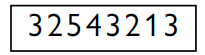
\includegraphics{Images/queens_position.png}
        \centering
    \end{frame}

    \begin{frame}
    \frametitle{Adjacent state: implementation}
        \begin{itemize}
            \item An adjacent state corresponds to a movement of the queen in her column.
            \pause
            \item For each column c (i.e. position in the list), for each row r (i.e. value of an element in that position): 
            \pause
            \begin{itemize}
                \item if queen in the column c is not in position r, a neighbor is represent by the same list with the new element r in position c.
            \end{itemize}
        \end{itemize}
    \end{frame}

    \begin{frame}
    \frametitle{Heuristics function: implementation}
        
    \end{frame}
\end{document}
